\documentclass[11pt,letterpaper]{article}
\input{glyphtounicode}
\pdfgentounicode=1
\usepackage[utf8]{inputenc}
\usepackage[T1]{fontenc}
\usepackage{lmodern}
\usepackage[spanish,es-noindentfirst,es-tabla]{babel}
\decimalpoint
\usepackage[margin=2.5cm]{geometry}
\usepackage{graphicx}
\usepackage{booktabs}
\usepackage{array}
\usepackage{multirow}
\usepackage{siunitx}
\sisetup{output-decimal-marker={.}, group-digits=false, detect-weight=true, table-number-alignment=center}
\usepackage{amsmath,amssymb}
\usepackage{listings}
\renewcommand{\lstlistingname}{Código}
\usepackage{xcolor}
\usepackage{tikz}
\usetikzlibrary{positioning,arrows.meta,shapes.geometric}
\usepackage{fancyhdr}
\usepackage{titlesec}
\usepackage{caption}
\usepackage[section]{placeins}
\usepackage[hidelinks]{hyperref}
\graphicspath{{figuras/}}
\renewcommand{\topfraction}{0.92}
\renewcommand{\bottomfraction}{0.85}
\renewcommand{\textfraction}{0.06}
\renewcommand{\floatpagefraction}{0.80}
\setcounter{topnumber}{3}
\setcounter{totalnumber}{5}
\captionsetup{font=small,labelfont=bf,textfont=it,labelsep=newline,justification=raggedright,singlelinecheck=false,skip=4pt}
\newcommand{\nota}[1]{\par\vspace{2pt}{\footnotesize\raggedright\textit{Nota.} #1\par}}

\lstdefinestyle{codigo}{
    language=Python,
    basicstyle=\ttfamily\footnotesize,
    keywordstyle=\color{blue!60!black}\bfseries,
    commentstyle=\color{gray},
    stringstyle=\color{orange!70!black},
    numbers=left,
    numberstyle=\tiny\color{gray},
    frame=single,
    breaklines=true,
    showstringspaces=false,
    tabsize=4,
    backgroundcolor=\color{gray!5},
    extendedchars=true,
    columns=fullflexible,
    keepspaces=true,
    literate={á}{{\'a}}1 {é}{{\'e}}1 {í}{{\'i}}1 {ó}{{\'o}}1 {ú}{{\'u}}1
             {Á}{{\'A}}1 {É}{{\'E}}1 {Í}{{\'I}}1 {Ó}{{\'O}}1 {Ú}{{\'U}}1
             {ñ}{{\~n}}1 {Ñ}{{\~N}}1 {¿}{{?`}}1 {¡}{{!`}}1 {±}{{$\pm$}}1
}
\lstset{style=codigo}

\pagestyle{fancy}
\fancyhf{}
\rhead{Inteligencia Computacional Aplicada}
\cfoot{\thepage}
\renewcommand{\headrulewidth}{0.4pt}
\titleformat{\section}{\normalfont\Large\bfseries}{\thesection.}{0.5em}{}
\titleformat{\subsection}{\normalfont\large\bfseries}{\thesubsection}{0.5em}{}

\newcommand{\nombreEstudiante}{Sergio Santiago Duarte Rojas}
\newcommand{\codigoEstudiante}{20261595002}
\newcommand{\nombreDocente}{Cesar Andrey Perdomo Charry}
\newcommand{\nombreAsignatura}{Inteligencia Computacional Aplicada}


\usepackage{xurl}
\graphicspath{{figuras/}}
\hypersetup{pdftitle={Series de tiempo. Taller 2, benchmarking de SARIMAX y NARX sobre PM2.5 en Beijing}, pdfauthor={Sergio Santiago Duarte Rojas}}
\lhead{Series de tiempo, Taller 2}
\setlength{\headheight}{14pt}

\begin{document}

\begin{titlepage}
    \centering
    \vspace*{2cm}
    {\LARGE \bfseries Series de tiempo. Taller 2\\[4pt] Benchmarking de SARIMAX y NARX sobre la concentración diaria de PM2.5 en Beijing\par}
    \vspace{0.5cm}
    {\large Informe\par}
    \vspace{2cm}
    \begin{tabular}{ll}
        \textbf{Asignatura:} & \nombreAsignatura \\
        \textbf{Docente:}    & \nombreDocente \\
        \textbf{Estudiante:} & \nombreEstudiante \\
        \textbf{Código:}     & \codigoEstudiante \\
        \textbf{Fecha:}      & 4 de noviembre de 2026 \\
    \end{tabular}
    \vfill
    Universidad Distrital Francisco José de Caldas
\end{titlepage}

\tableofcontents
\newpage

\section{Introducción}

Este informe compara un ingenuo estacional, un SARIMAX y una red NARX en el pronóstico a 24 días de la concentración media diaria de PM2.5 de la estación Aotizhongxin, con temperatura, punto de rocío, presión y velocidad del viento como exógenas. Los hiperparámetros se eligieron por validación cruzada de origen móvil dentro del bloque de desarrollo, y la prueba externa se evaluó una sola vez al final. En la prueba externa la raíz del error cuadrático medio fue de 96.2 para el ingenuo, 70.2 para SARIMAX y 44.0 para NARX, y la diferencia entre SARIMAX y NARX es significativa ($p=0.003$). La ventaja de la red proviene de su uso de la meteorología, porque sin exógenas los dos modelos alcanzan el mismo error en desarrollo.

\section{Marco teórico (resumen)}

SARIMAX combina una estructura ARIMA estacional con una regresión lineal sobre variables exógenas (Box et al., 2015). Su pronóstico a varios pasos converge, al alejarse del origen, a la media condicionada por las exógenas, y su efecto sobre la serie es lineal en la escala en que se modela. La red NARX aproxima la relación entre los retardos de la salida y de las exógenas con un perceptrón multicapa (Leontaritis y Billings, 1985). En lazo cerrado cada predicción entra como retardo de la siguiente. El error se propaga así a lo largo del horizonte, más cuanto mayor es el peso que la red da a los retardos de la salida.

Cuando el modelo se ajusta sobre $z=\log(1+y)$ con error aproximadamente normal, $\exp(\hat z)$ estima la mediana y no la media. La transformación inversa $\exp(\hat z+\hat\sigma^2/2)-1$ corrige ese sesgo. La fuerza de la tendencia $F_T$ y de la estacionalidad $F_S$ se calcula a partir de la descomposición STL y toma valores entre 0 y 1 (Hyndman y Athanasopoulos, 2021). La validación cruzada de origen móvil entrena con la historia anterior a cada origen y evalúa el bloque siguiente, lo que respeta el orden temporal (Bergmeir y Benítez, 2012). La prueba de Diebold y Mariano (1995) con la corrección de Harvey et al. (1997) compara la pérdida cuadrática de dos modelos, y un estadístico positivo favorece al segundo del par. La prueba de Ljung y Box (1978) evalúa la autocorrelación remanente en los residuos.

\section{Metodología}

\subsection{Datos y validación previa}

Los datos son los registros horarios de la estación Aotizhongxin entre el 1 de marzo de 2013 y el 28 de febrero de 2017, publicados en el repositorio UCI (Chen, 2017) y descritos por Zhang et al. (2017). El cuaderno los agrega a promedios diarios, lo que da 1461 días, e imputa por interpolación temporal 15 días sin dato de PM2.5. El 80~\% inicial (1168 días, hasta el 11 de mayo de 2016) forma el bloque de desarrollo y los 293 días restantes la prueba externa. La Tabla~\ref{tab:validacion} reúne los criterios de validación del cuaderno.

\begin{table}[!htb]
    \centering
    \caption{Validación previa del conjunto de datos}
    \label{tab:validacion}
    \footnotesize
    \begin{tabular}{l l c}
        \toprule
        \textbf{Criterio} & \textbf{Evidencia} & \textbf{Cumple} \\
        \midrule
        C1 Índice monótono y sin duplicados & verificación automática del cuaderno & sí \\
        C2 Muestreo regular & paso modal de una hora & sí \\
        C3 Faltantes en el objetivo $\le 10$~\% & 2.64~\% de horas sin PM2.5 & sí \\
        C4 Longitud $\ge 10$ periodos estacionales & 1461 días frente a 70 & sí \\
        C5 Exógenas existentes y numéricas & TEMP, DEWP, PRES y WSPM & sí \\
        C6 Objetivo no constante & desviación positiva & sí \\
        C7 Origen, licencia y unidades & UCI, CC BY 4.0, \textmu g/m$^3$, \textdegree C, hPa y m/s & sí \\
        C8 Exógenas disponibles al pronosticar & pronóstico meteorológico a 24 días, supuesto conocido & con reserva \\
        \bottomrule
    \end{tabular}
    \nota{C7 y C8 se documentan de forma manual. La reserva de C8 se discute en el análisis.}
\end{table}

\subsection{Diagnóstico y decisiones de diseño}

En el bloque de desarrollo las pruebas ADF ($p<0.001$) y KPSS ($p\ge0.10$) coinciden en que la serie es estacionaria en nivel, por lo que no se diferencia ($d=D=0$). La fuerza de la estacionalidad semanal es baja ($F_S=0.071$), igual que la de la tendencia ($F_T=0.200$). Entre las exógenas, la velocidad del viento es la de mayor correlación con PM2.5 ($r=-0.38$). La serie tiene una cola derecha extensa, con días por encima de 400~\textmu g/m$^3$, y ambos modelos trabajan sobre $\log(1+y)$ con la corrección de sesgo de la transformación inversa.

Antes de definir las rejillas se compararon variantes de diseño con la misma validación cruzada (Tabla~\ref{tab:diseno}). En SARIMAX el criterio de Akaike favorece el orden $(3,0,0)$, pero ese orden produce un error medio de 92.9 en la validación cruzada, por pronósticos inestables, y se descartó como punto de partida.

\begin{table}[!htb]
    \centering
    \caption{Raíz del error cuadrático medio en la validación cruzada de las variantes de diseño}
    \label{tab:diseno}
    \footnotesize
    \begin{tabular}{l c c}
        \toprule
        \textbf{Variante} & \textbf{SARIMAX $(1,0,1)$} & \textbf{NARX $d_y=3$, 8 neuronas} \\
        \midrule
        Diseño adoptado & 49.95 & 38.84 \\
        Sin exógenas & 57.77 & 57.11 \\
        Sin logaritmo & 51.83 & 43.78 \\
        Sin corrección de sesgo & 50.79 & \textendash \\
        Solo exógenas contemporáneas ($d_x=0$) & \textendash & 41.66 \\
        \bottomrule
    \end{tabular}
    \nota{El diseño adoptado usa el logaritmo, las cuatro exógenas y la corrección de sesgo. Cinco pliegues de origen móvil dentro del bloque de desarrollo, horizonte de 24 días. NARX con semilla 2026.}
\end{table}

\subsection{Modelos, rejillas y selección}

El modelo clásico es un SARIMAX con constante sobre $\log(1+y)$ y las cuatro exógenas como regresores, ajustado con statsmodels (Seabold y Perktold, 2010). La red NARX recibe $\log(1+y)$ en los retardos $1,\dots,d_y$ y las exógenas en $t$ y $t-1$ ($d_x=1$), estandarizadas con la media y la desviación del entrenamiento de cada pliegue. Tiene una capa oculta $\tanh$, regularización $L_2=10^{-4}$ y optimizador Adam, con parada temprana (paciencia de 30 épocas) sobre el 15~\% final del entrenamiento del pliegue. La varianza de los residuos de ese tramo alimenta la corrección de sesgo. El pronóstico se construye en lazo cerrado.

Las rejillas cruzan tres órdenes no estacionales $\{(1,0,0),(1,0,1),(2,0,1)\}$ con tres partes estacionales $\{\text{ninguna},(1,0,0)_7,(1,0,1)_7\}$ en SARIMAX, y $d_y\in\{1,3,7\}$ con $\{4,8,16\}$ neuronas y las semillas 1, 2 y 3 en NARX. Cada combinación se evalúa en cinco pliegues de ventana expandible con orígenes en el 40~\% final del desarrollo y horizonte de 24 días. Se elige la combinación de menor error medio, y en la red ese error se promedia sobre las tres semillas. Los modelos elegidos se evalúan después en 12 orígenes de la prueba externa.

\section{Resultados}

La selección fijó SARIMAX $(1,0,1)$ sin parte estacional y NARX con $d_y=1$ y 8 neuronas. La Figura~\ref{fig:sensibilidad} muestra las dos superficies de sensibilidad y la Tabla~\ref{tab:benchmark} las métricas en la validación cruzada y en la prueba externa.

\begin{figure}[!htb]
    \centering
    \caption{Raíz del error cuadrático medio en la validación cruzada según los hiperparámetros}
    \label{fig:sensibilidad}
    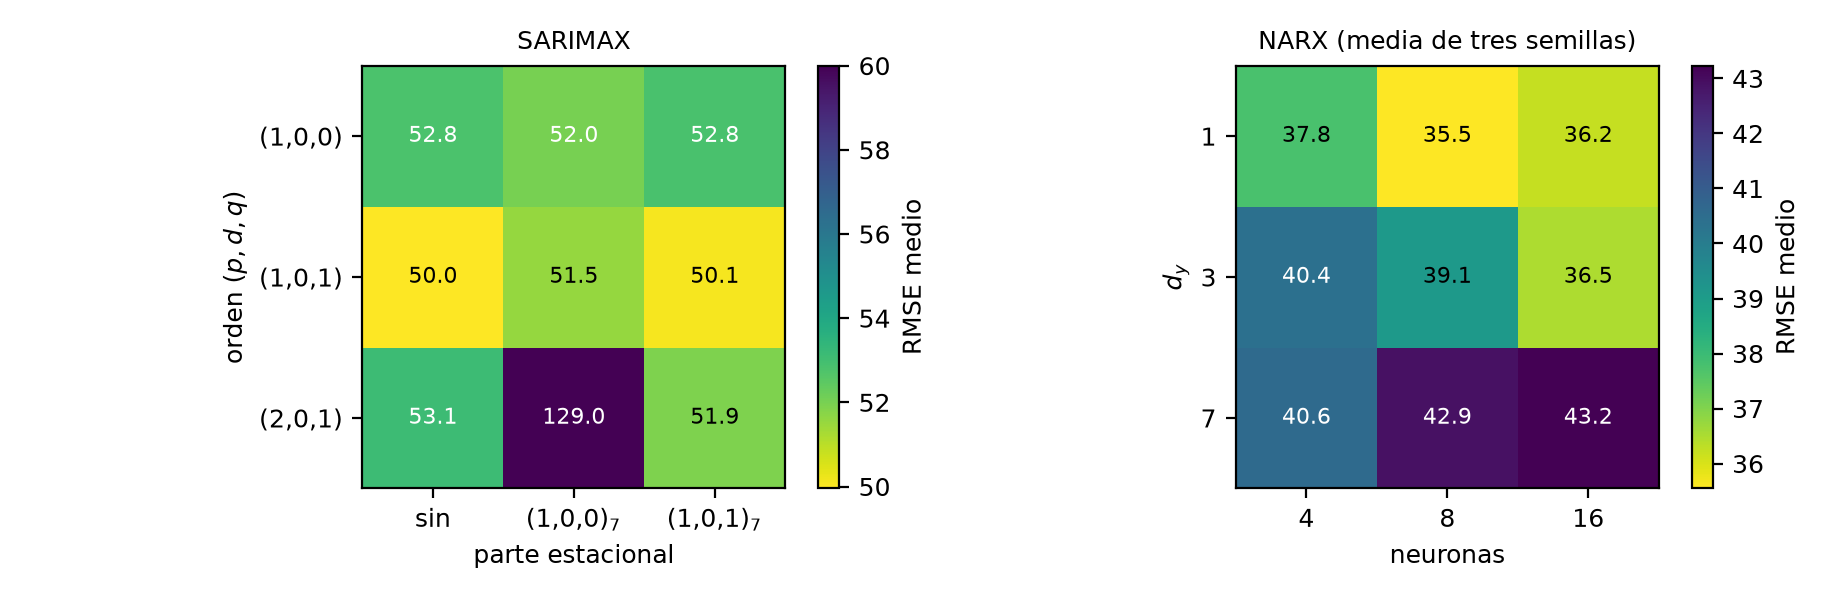
\includegraphics[width=15.5cm]{fig01_sensibilidad.png}
    \nota{La escala de SARIMAX se corta en 60 para que la combinación inestable no oculte las demás diferencias.}
\end{figure}

\begin{table}[!htb]
    \centering
    \caption{Métricas de los modelos elegidos en la validación cruzada y en la prueba externa}
    \label{tab:benchmark}
    \footnotesize
    \setlength{\tabcolsep}{4.5pt}
    \begin{tabular}{l c c c c c c c c}
        \toprule
        & \multicolumn{4}{c}{\textbf{Validación cruzada}} & \multicolumn{4}{c}{\textbf{Prueba externa}} \\
        \cmidrule(lr){2-5}\cmidrule(lr){6-9}
        \textbf{Modelo} & RMSE & MAE & MAPE & MASE & RMSE & MAE & MAPE & MASE \\
        \midrule
        Ingenuo estacional & 110.53 & 71.69 & 194.2 & 1.005 & 96.24 & 69.49 & 175.6 & 0.974 \\
        SARIMAX $(1,0,1)$ & 51.47 & 37.06 & 109.2 & 0.519 & 70.18 & 49.63 & 110.6 & 0.696 \\
        NARX $d_y=1$, 8 neuronas & 40.07 & 28.81 & 80.0 & 0.404 & 44.02 & 28.75 & 53.5 & 0.403 \\
        \bottomrule
    \end{tabular}
    \nota{MAPE en porcentaje. MASE escalado con el error del ingenuo estacional en el bloque de desarrollo. La red final usa la semilla 2026 del cuaderno.}
\end{table}

\begin{figure}[!htb]
    \centering
    \caption{Raíz del error cuadrático medio por horizonte en la prueba externa}
    \label{fig:horizonte}
    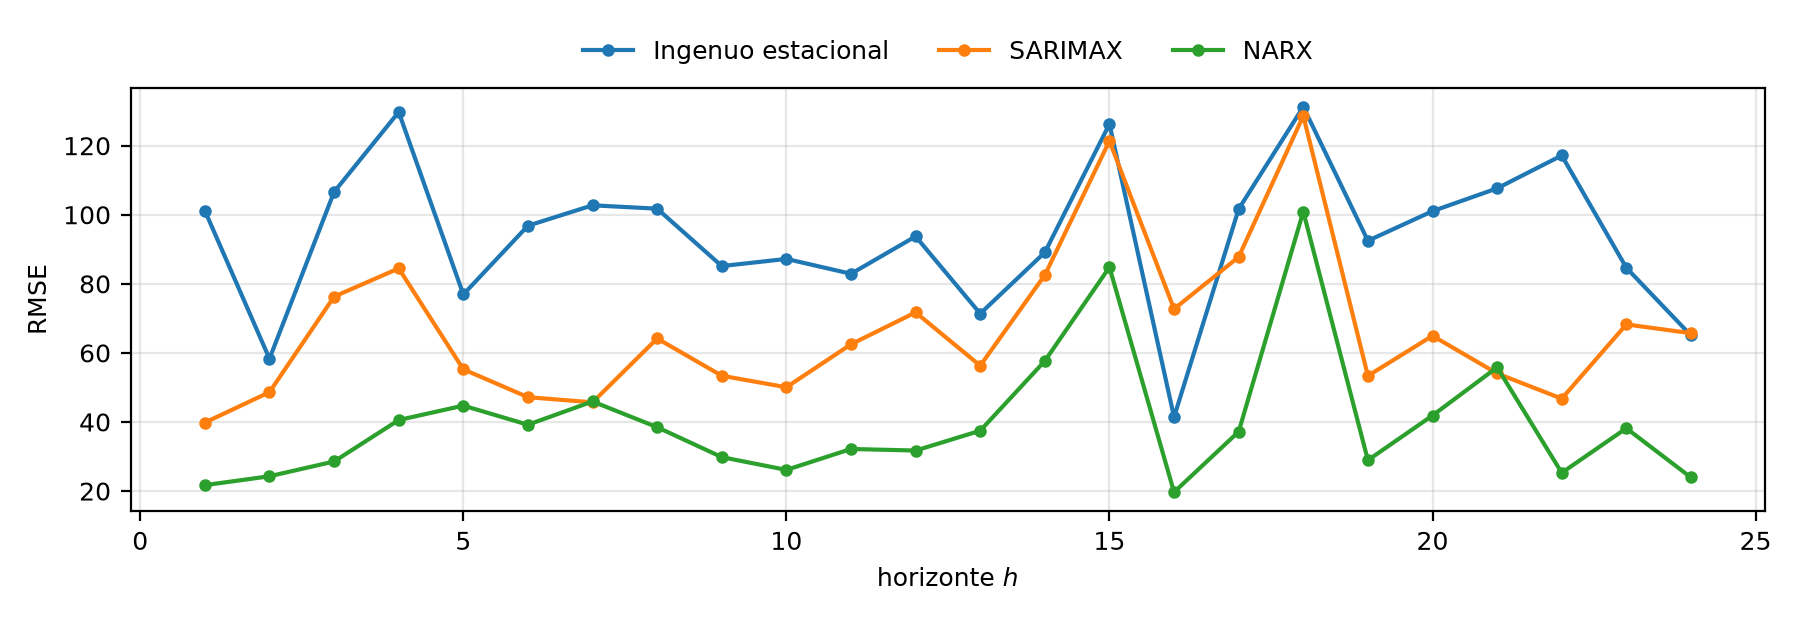
\includegraphics[width=14cm]{fig02_rmse_horizonte.png}
    \nota{Cada punto promedia los 12 orígenes de la prueba externa.}
\end{figure}

En la prueba de Diebold y Mariano a 24 pasos, NARX supera a SARIMAX (DM*$=2.98$, $p=0.003$) y al ingenuo (DM*$=2.43$, $p=0.016$), mientras que la diferencia entre el ingenuo y SARIMAX no es significativa al 5~\% (DM*$=1.74$, $p=0.083$). La prueba de Ljung y Box en el retardo 7 rechaza la ausencia de autocorrelación en los tres modelos, con estadísticos de 102.3 para el ingenuo, 437.3 para SARIMAX y 110.8 para NARX.

\begin{figure}[!htb]
    \centering
    \caption{Residuos de SARIMAX (arriba) y de NARX (abajo) en la prueba externa}
    \label{fig:residuos}
    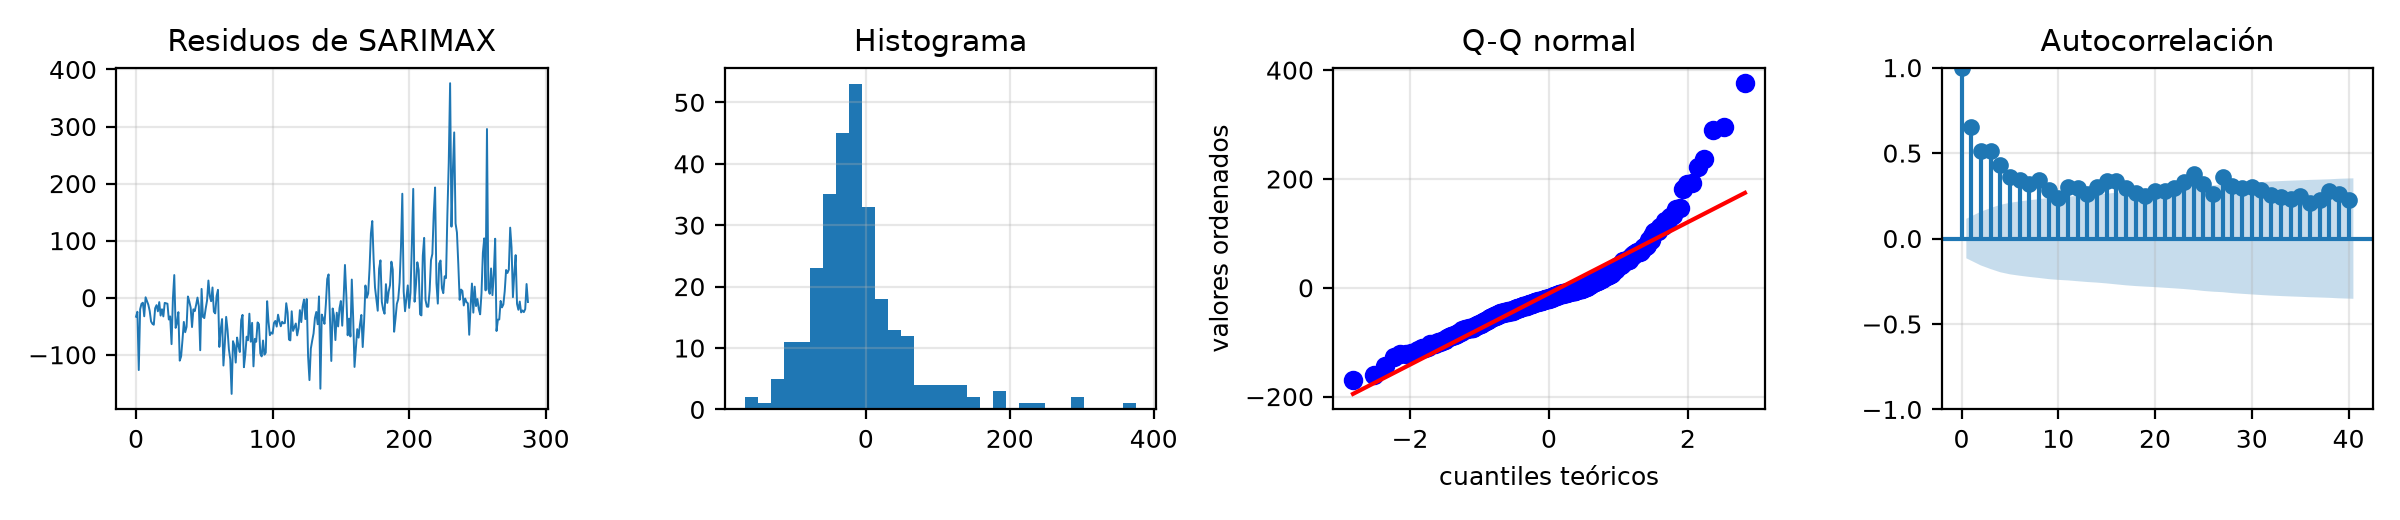
\includegraphics[width=15.5cm]{fig03a_residuos_sarimax.png}\\
    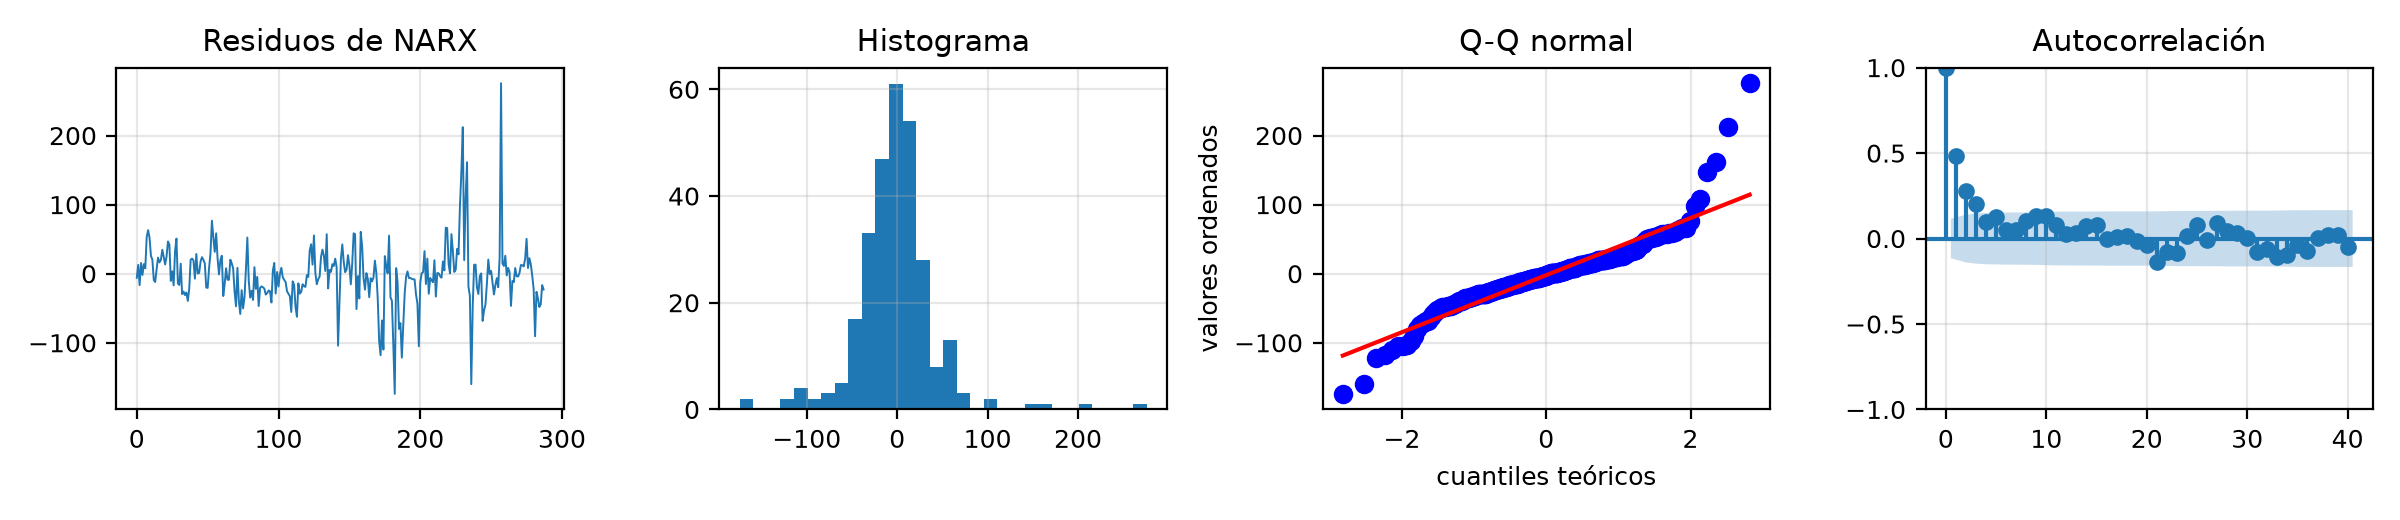
\includegraphics[width=15.5cm]{fig03b_residuos_narx.png}
    \nota{Residuos de los 12 orígenes concatenados en orden temporal. El residuo es el valor observado menos el pronóstico.}
\end{figure}

\section{Análisis}

\subsection{Origen de la ventaja de la red}

Sin exógenas, SARIMAX y NARX obtienen 57.8 y 57.1 en la validación cruzada (Tabla~\ref{tab:diseno}). Con la sola historia de PM2.5 ninguna estructura saca ventaja. Con las mismas cuatro exógenas, SARIMAX baja a 50.0 y la red a 38.8. La diferencia está en el uso de la meteorología. En SARIMAX el efecto de cada variable es un coeficiente constante sobre el logaritmo, y en la red depende del valor de las demás entradas. El retardo de un día en las exógenas reduce el error de la red de 41.7 a 38.8. El tiempo del día anterior pesa sobre la concentración de hoy, como documentan Zhang et al. (2017) para esta red de estaciones. El logaritmo también favorece más a la red (de 43.8 a 38.8) que a SARIMAX (de 51.8 a 50.0), porque reduce el rango de la variable de salida que la capa $\tanh$ debe cubrir.

El mismo hecho explica por qué $d_y=1$ resultó el mejor número de retardos. En lazo cerrado, con un solo retardo de la salida, el pronóstico se apoya en la meteorología futura después de pocos pasos, y el error de NARX por horizonte no crece de forma sostenida (Figura~\ref{fig:horizonte}). Esto también señala la principal reserva del estudio (criterio C8). El cuaderno supone conocida la meteorología de los 24 días siguientes. En operación, esas entradas provendrían de un pronóstico meteorológico con error propio, que crece con el horizonte y afectaría más a la red, cuya ventaja depende de ellas. Las cifras de la prueba son una cota optimista.

\subsection{Sensibilidad de los hiperparámetros}

La superficie de SARIMAX es plana, con errores entre 50.0 y 53.1 en ocho de las nueve combinaciones (Figura~\ref{fig:sensibilidad}). La parte estacional no mejora el ajuste, porque $(1,0,1)$ con $(1,0,1)_7$ obtiene 50.1 frente a 50.0 sin ella, coherente con $F_S=0.071$. La combinación $(2,0,1)$ con $(1,0,0)_7$ alcanza 129.0 con una desviación entre pliegues de 152.7, señal de que la predicción diverge en alguno de los pliegues. Lo mismo ocurrió con el orden $(3,0,0)$ que eligió el criterio de Akaike. Un buen ajuste dentro de la muestra no garantizó un pronóstico estable a 24 días, y la validación cruzada lo detectó.

En la red, $d_y$ es el factor dominante. Con un retardo el error medio queda entre 35.5 y 37.8, y con siete entre 40.6 y 43.2. El número de neuronas interactúa con los retardos. Con $d_y=1$ y $d_y=3$, pasar de 4 a 16 neuronas reduce el error, y con $d_y=7$ lo aumenta, porque más entradas y más neuronas elevan la varianza del estimador sin que los retardos lejanos aporten información, dada la estacionalidad semanal débil. La desviación entre semillas va de 0.1 a 2.8. La red final, entrenada con la semilla 2026 del cuaderno, obtiene 40.1 en la validación cruzada frente a la media de 35.5 de las tres semillas de la rejilla. Esa dispersión es mayor que la diferencia entre las tres mejores combinaciones (35.5, 36.2 y 36.5), cuyo orden no queda establecido, pero es menor que la distancia de cerca de diez unidades o más que separa cualquier configuración de NARX con $d_y\le3$ del mejor SARIMAX.

\subsection{Prueba externa y residuos}

SARIMAX empeora de 51.5 en la validación cruzada a 70.2 en la prueba, un aumento del 36~\%, mientras que NARX pasa de 40.1 a 44.0 y conserva el mismo error absoluto medio (28.8). Los residuos de SARIMAX son negativos en la primera mitad de la prueba, que corresponde a los meses de verano y otoño de 2016 con concentraciones bajas, y grandes y positivos en los episodios del invierno siguiente (Figura~\ref{fig:residuos}). Su autocorrelación se mantiene entre 0.25 y 0.5 hasta el retardo 40. El modelo sobrestima los periodos limpios y subestima los episodios, y ese error persistente explica también su MAPE de 110.6~\%, que penaliza la sobrestimación en niveles bajos, frente al 53.5~\% de la red.

Los residuos de NARX solo muestran autocorrelación significativa en los tres primeros retardos. Con pronósticos a 24 pasos desde un mismo origen esa dependencia corta es esperable, porque los errores de horizontes consecutivos comparten la información disponible en el origen. Por eso Ljung y Box rechaza en los tres modelos. La comparación útil es la magnitud del estadístico, cuatro veces mayor en SARIMAX que en NARX. La misma persistencia explica que la diferencia entre el ingenuo y SARIMAX no resulte significativa pese a 96.2 frente a 70.2, ya que la prueba de Diebold y Mariano con horizonte 24 estima la varianza de largo plazo con 23 autocovarianzas y los errores autocorrelacionados la inflan.

En la Figura~\ref{fig:horizonte}, los máximos en $h=15$ y $h=18$ son comunes a los tres modelos. Con 12 orígenes, el error de cada horizonte queda dominado por unos pocos días, y esos máximos corresponden a episodios que ningún modelo anticipó, no a un deterioro con el horizonte. En costo, NARX requiere cerca de 50 veces el tiempo de SARIMAX (141.6 frente a 2.7~s en la validación cruzada).

\section{Conclusiones}

En esta serie la estacionalidad semanal es débil y la información predictiva está en la meteorología. Elegir modelo es elegir cómo se usan las exógenas. NARX con un retardo de la salida y ocho neuronas supera a SARIMAX en la validación cruzada y en la prueba externa con diferencia significativa, y mantiene su error fuera del periodo de desarrollo, mientras que SARIMAX acumula errores persistentes por estación. Sin exógenas ambos modelos se igualan.

La validación cruzada descartó órdenes que el criterio de Akaike favorecía y que producen pronósticos inestables a 24 días. En la red, la variabilidad entre semillas impide ordenar las mejores combinaciones, aunque no altera la ventaja frente a SARIMAX. El supuesto de meteorología futura conocida hace de los resultados una cota optimista para un uso operativo.

\section{Declaración de uso de inteligencia artificial}

Se usó Claude como apoyo en la redacción, la revisión de consistencia entre conceptos y la preparación de tablas y gráficas. Los procedimientos, las modificaciones al código fuente y la estructura del documento son del autor, quien verificó cada cifra con las salidas del cuaderno.

\section{Referencias}

\begin{itemize}
    \setlength{\itemsep}{2pt}
    \item[] Bergmeir, C., \& Benítez, J. M. (2012). On the use of cross-validation for time series predictor evaluation. \textit{Information Sciences, 191}, 192--213. \url{https://doi.org/10.1016/j.ins.2011.12.028}
    \item[] Box, G. E. P., Jenkins, G. M., Reinsel, G. C., \& Ljung, G. M. (2015). \textit{Time series analysis: Forecasting and control} (5.ª ed.). Wiley.
    \item[] Chen, S. (2017). \textit{Beijing multi-site air quality} [Conjunto de datos]. UCI Machine Learning Repository. \url{https://doi.org/10.24432/C5RK5G}
    \item[] Diebold, F. X., \& Mariano, R. S. (1995). Comparing predictive accuracy. \textit{Journal of Business \& Economic Statistics, 13}(3), 253--263. \url{https://doi.org/10.1080/07350015.1995.10524599}
    \item[] Harvey, D., Leybourne, S., \& Newbold, P. (1997). Testing the equality of prediction mean squared errors. \textit{International Journal of Forecasting, 13}(2), 281--291. \url{https://doi.org/10.1016/S0169-2070(96)00719-4}
    \item[] Hyndman, R. J., \& Athanasopoulos, G. (2021). \textit{Forecasting: Principles and practice} (3.ª ed.). OTexts. \url{https://otexts.com/fpp3/}
    \item[] Leontaritis, I. J., \& Billings, S. A. (1985). Input-output parametric models for non-linear systems Part I: Deterministic non-linear systems. \textit{International Journal of Control, 41}(2), 303--328. \url{https://doi.org/10.1080/00207178508961129}
    \item[] Ljung, G. M., \& Box, G. E. P. (1978). On a measure of lack of fit in time series models. \textit{Biometrika, 65}(2), 297--303. \url{https://doi.org/10.1093/biomet/65.2.297}
    \item[] Seabold, S., \& Perktold, J. (2010). statsmodels: Econometric and statistical modeling with Python. En \textit{Proceedings of the 9th Python in Science Conference} (pp. 92--96). \url{https://doi.org/10.25080/Majora-92bf1922-011}
    \item[] Zhang, S., Guo, B., Dong, A., He, J., Xu, Z., \& Chen, S. X. (2017). Cautionary tales on air-quality improvement in Beijing. \textit{Proceedings of the Royal Society A, 473}(2205), 20170457. \url{https://doi.org/10.1098/rspa.2017.0457}
\end{itemize}

\end{document}
